e\chapter{Hardware}

% % \ref{fig:coordination-diagram}.

% \begin{figure} [H]
%     \centering
%     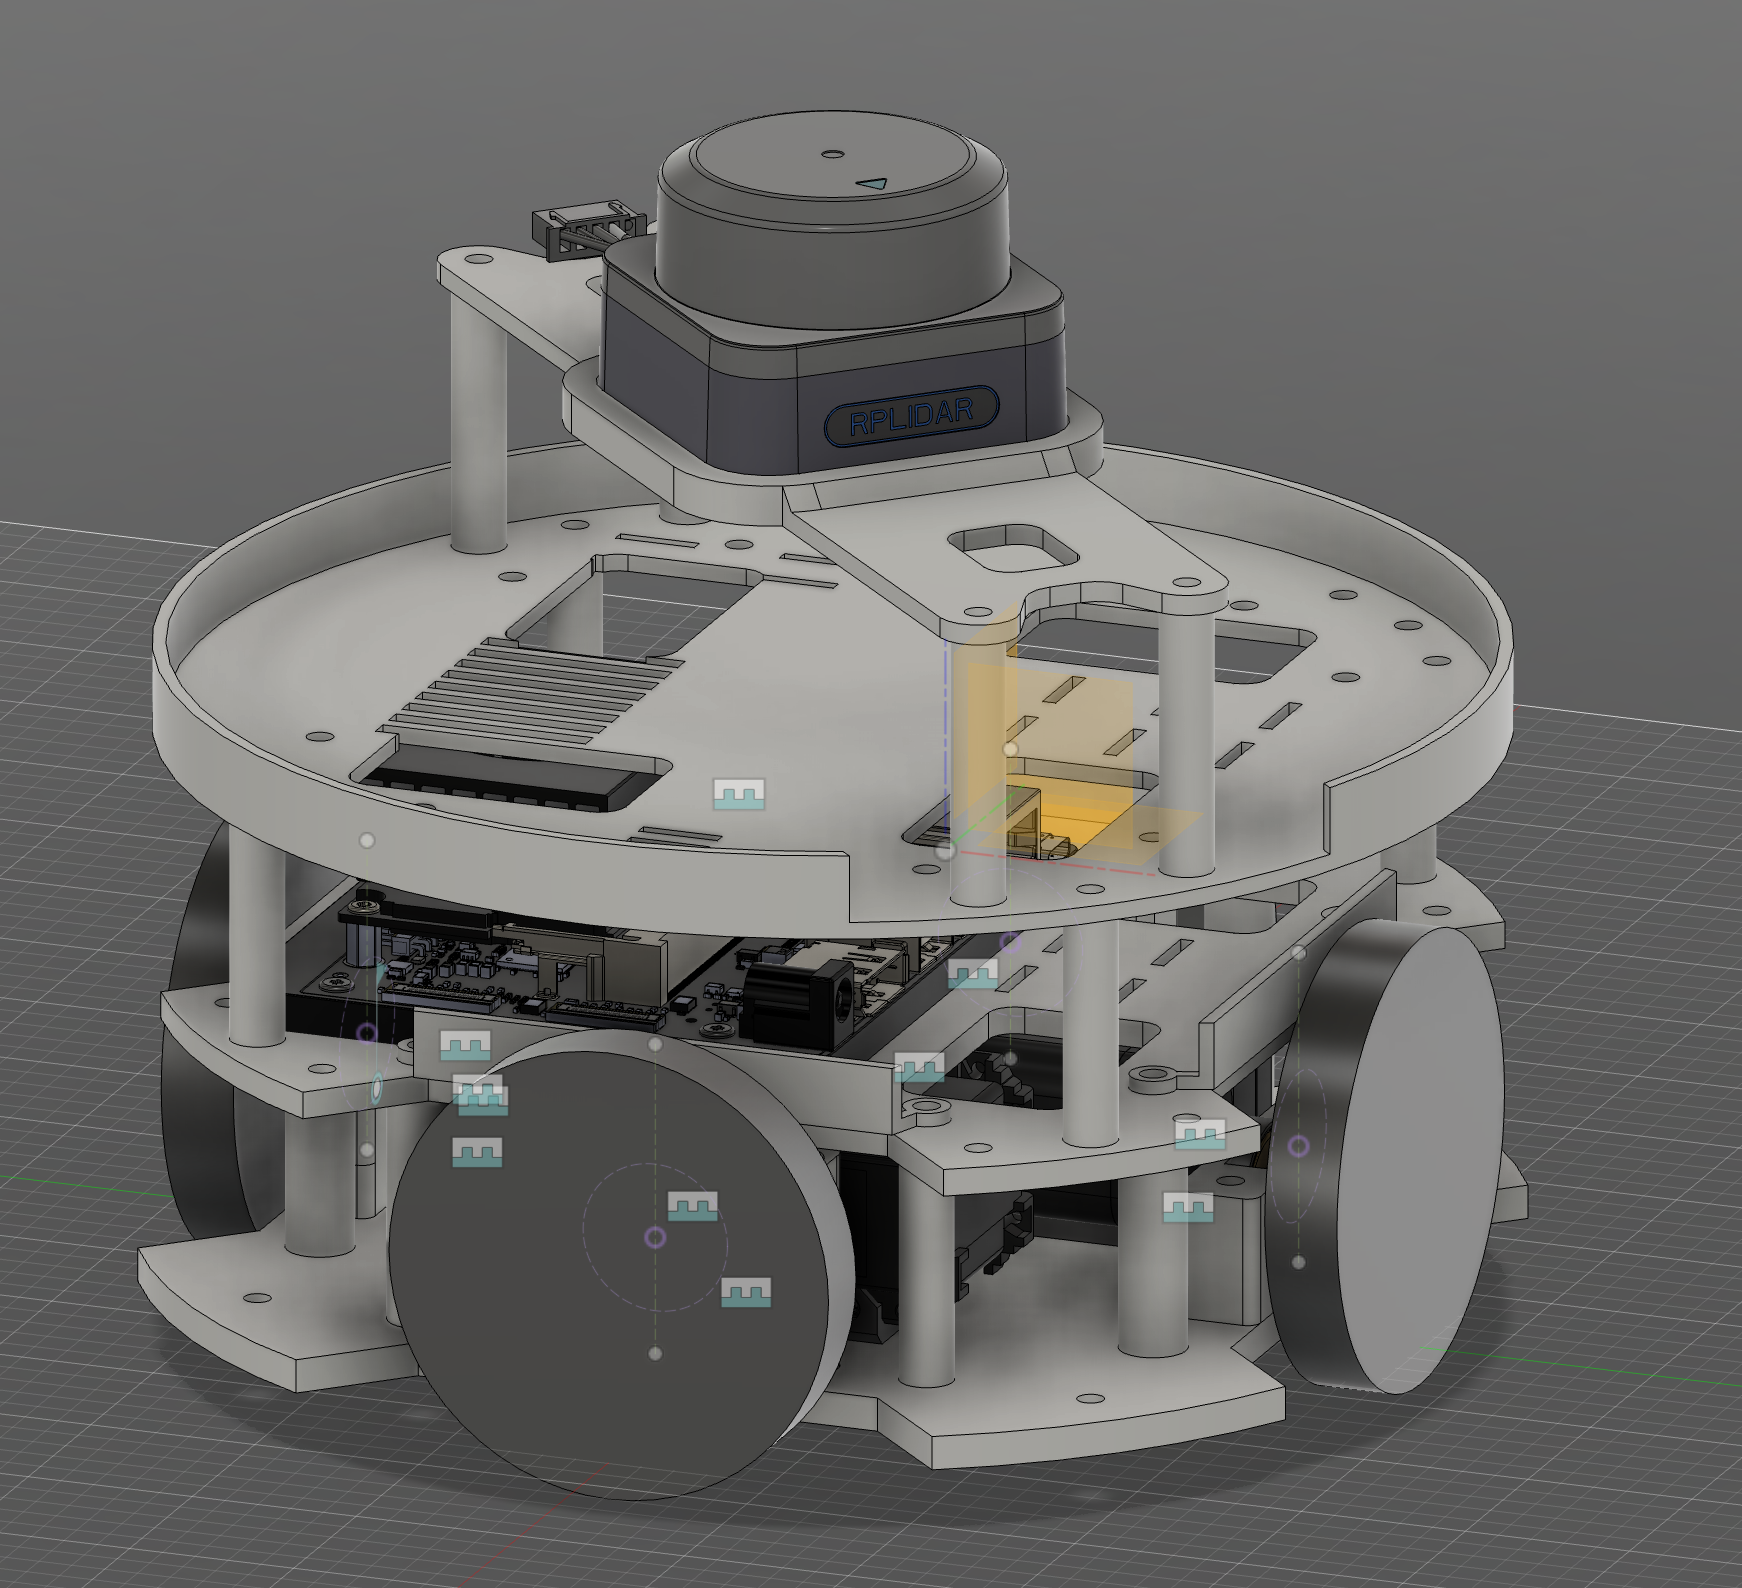
\includegraphics[width=0.65\linewidth]{assets/images/hardware/robotcad3layer.png}
%     \caption{Robot CAD model}
%     \label{fig:robo-cad}
% \end{figure}

\begin{figure} [H]
    \centering
    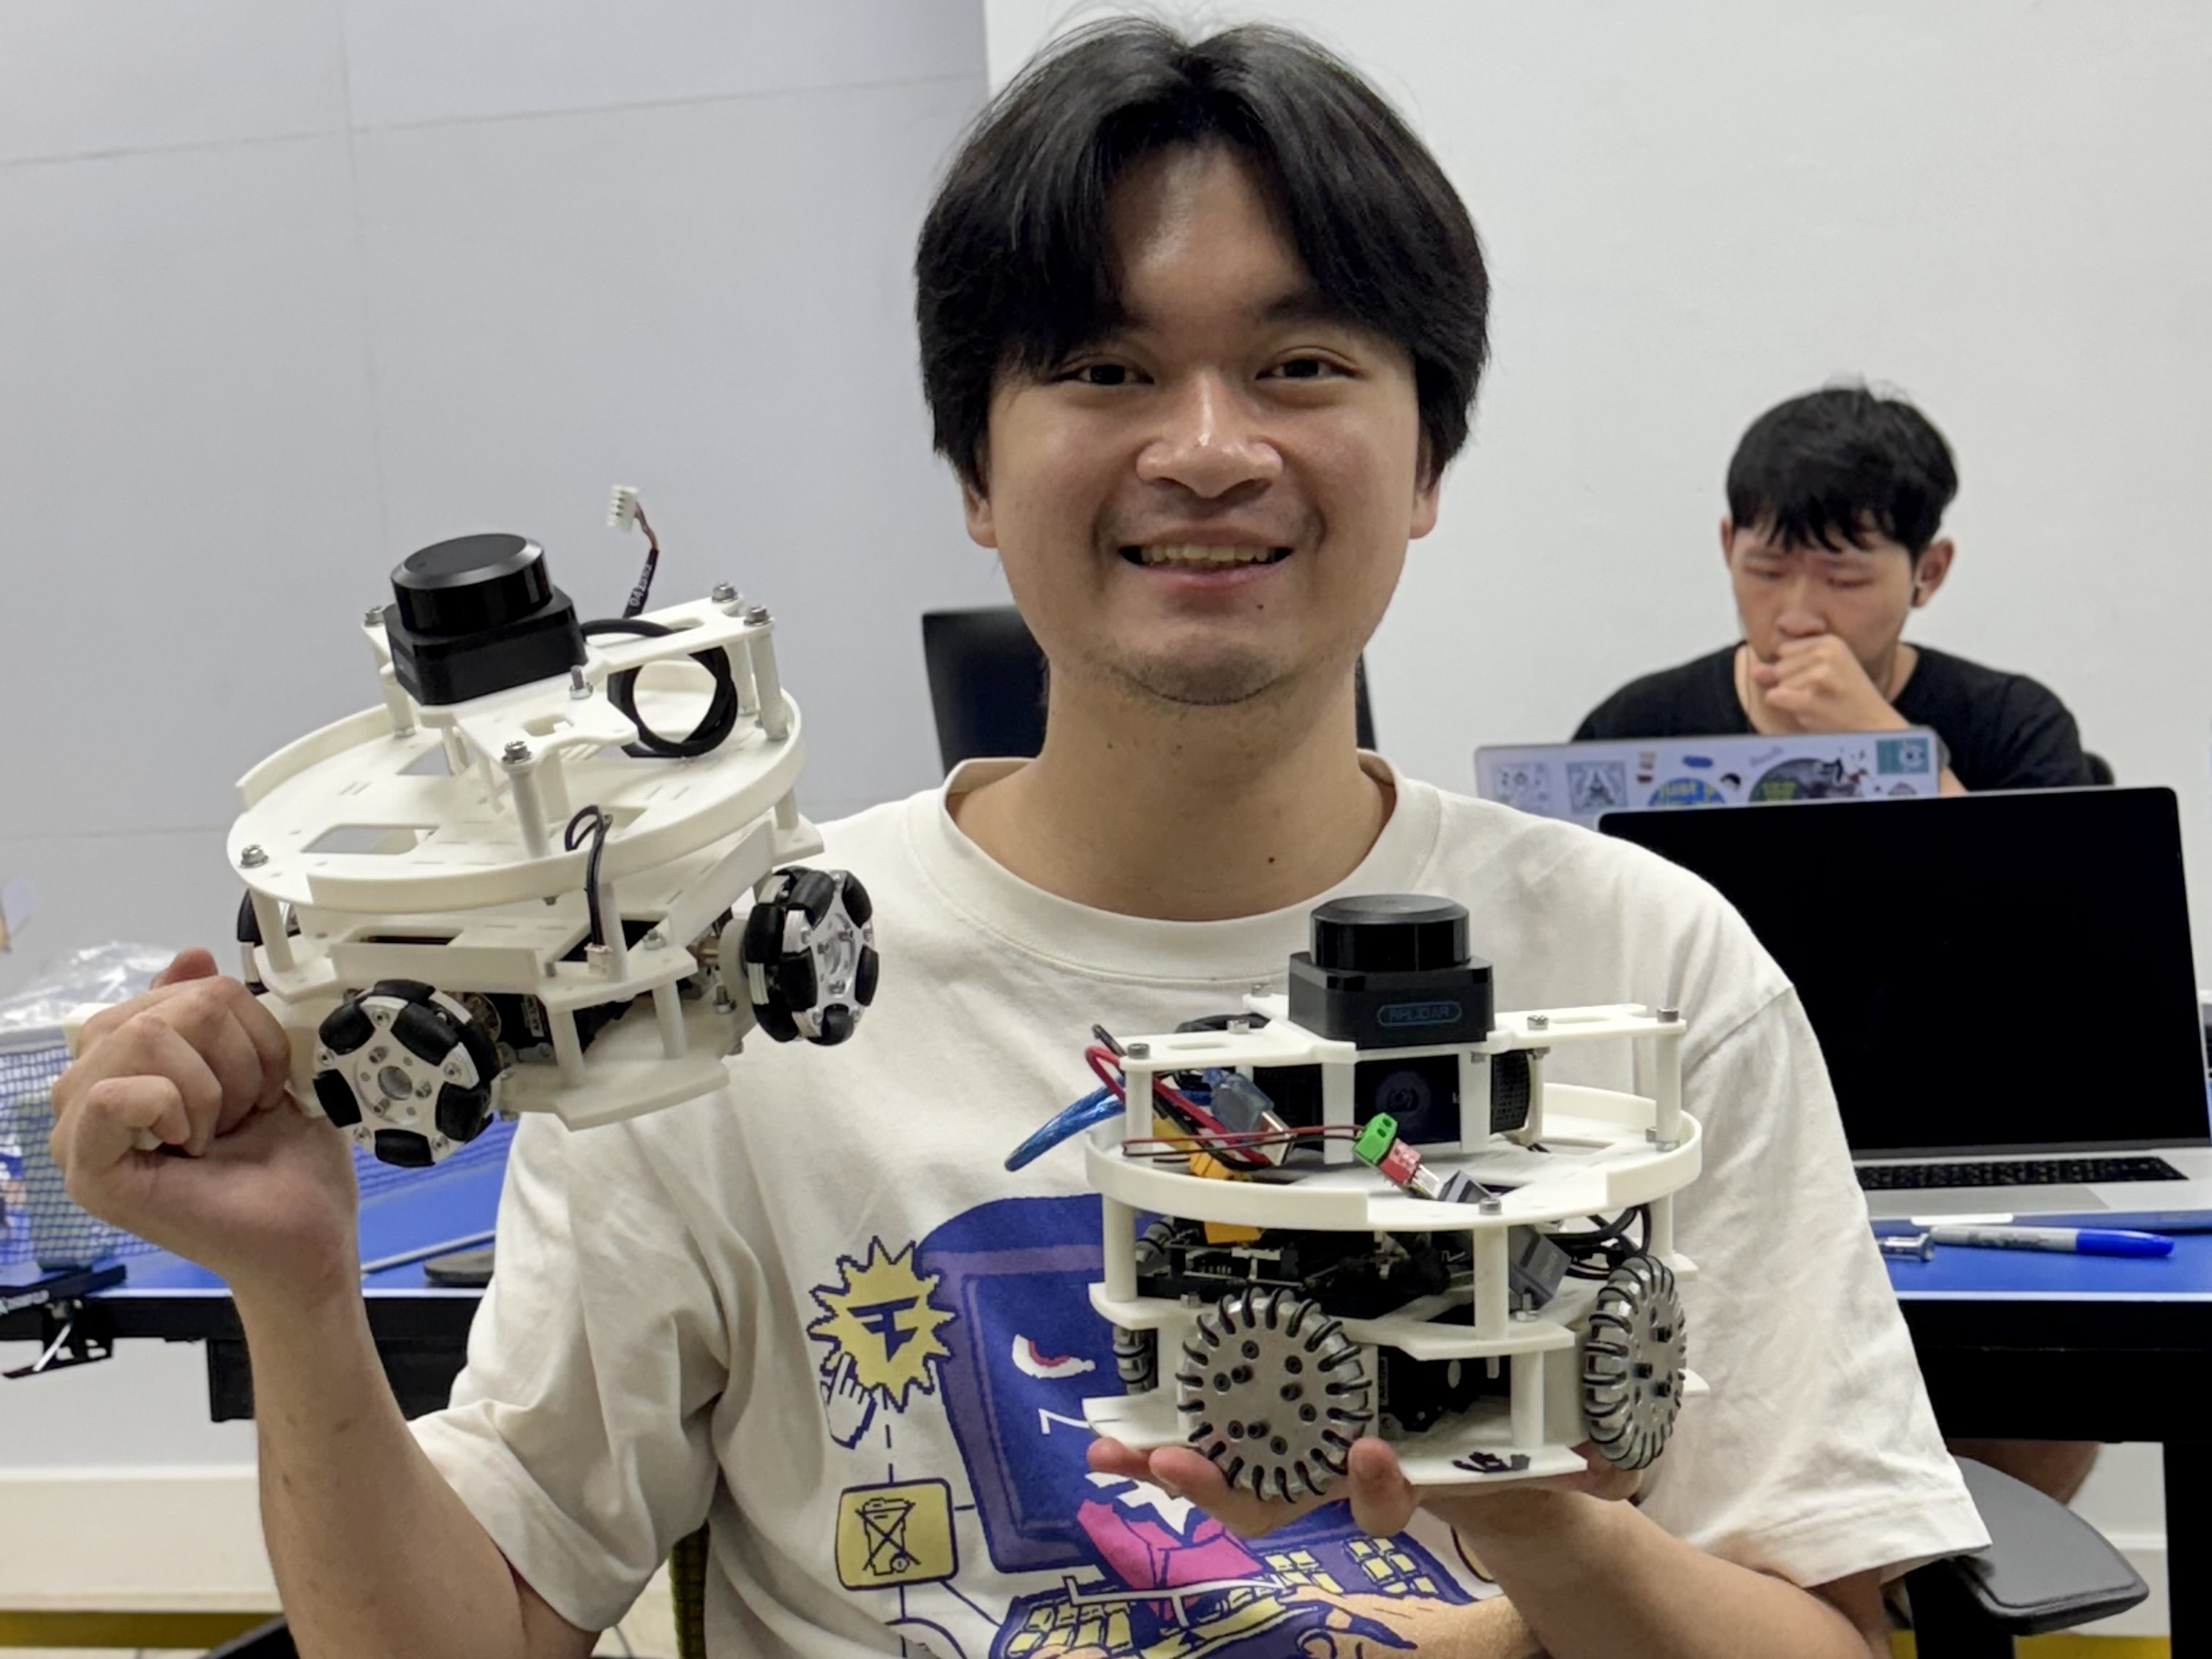
\includegraphics[width=0.65\linewidth]{assets/images/hardware/IMG_8290.jpeg}
    \caption{A happy man holding 2 built robots}
    \label{fig:have2robots}
\end{figure}
For hardware we have built the second robot with ease. Redesigning to encoporate metal parts were in order. the image on the left of the \ref{fig:metal-parts}, are 6mm metal shaft to replace the PLA 3D printed ones. The middle image is the robot with the metal shafts attached the motor with a 6mm flange coupler and the omni-wheel; A 6mm journal bearing is used to off-load the shear stress to motor, it's pressed-fit intoa a 3D printed pillow block as we couldn't find a machined parts in-time. The right image is the robot with the metal shafts attached and the wheels attached. 
The omni-wheel are now newly bought from a local supplier with thicker rubber which helps to reduce slip, much improved from the first robot, which had a lot of slip. The robot is now able to move in all directions with ease. Further testing are required to imperically prove the improvement. Despite the base still made from 5mm 3D printed PLA, it's quite rigid, we plan to change the plate to 5mm arcylic to test the rigidity of the base. As according to a paper, 3D printed PLA has a range of Young's modulus of 2.1 to 4.4 GPa GPa, while arcylic has a Young's modulus of 3.6 GPa. Therefore, hard to conclude with this better without proper testing. 

\begin{figure} [H]
    \centering
    \begin{tabular}{@{}c@{\hspace{0.5cm}}p{8cm}@{\hspace{0.5cm}}c@{}}
        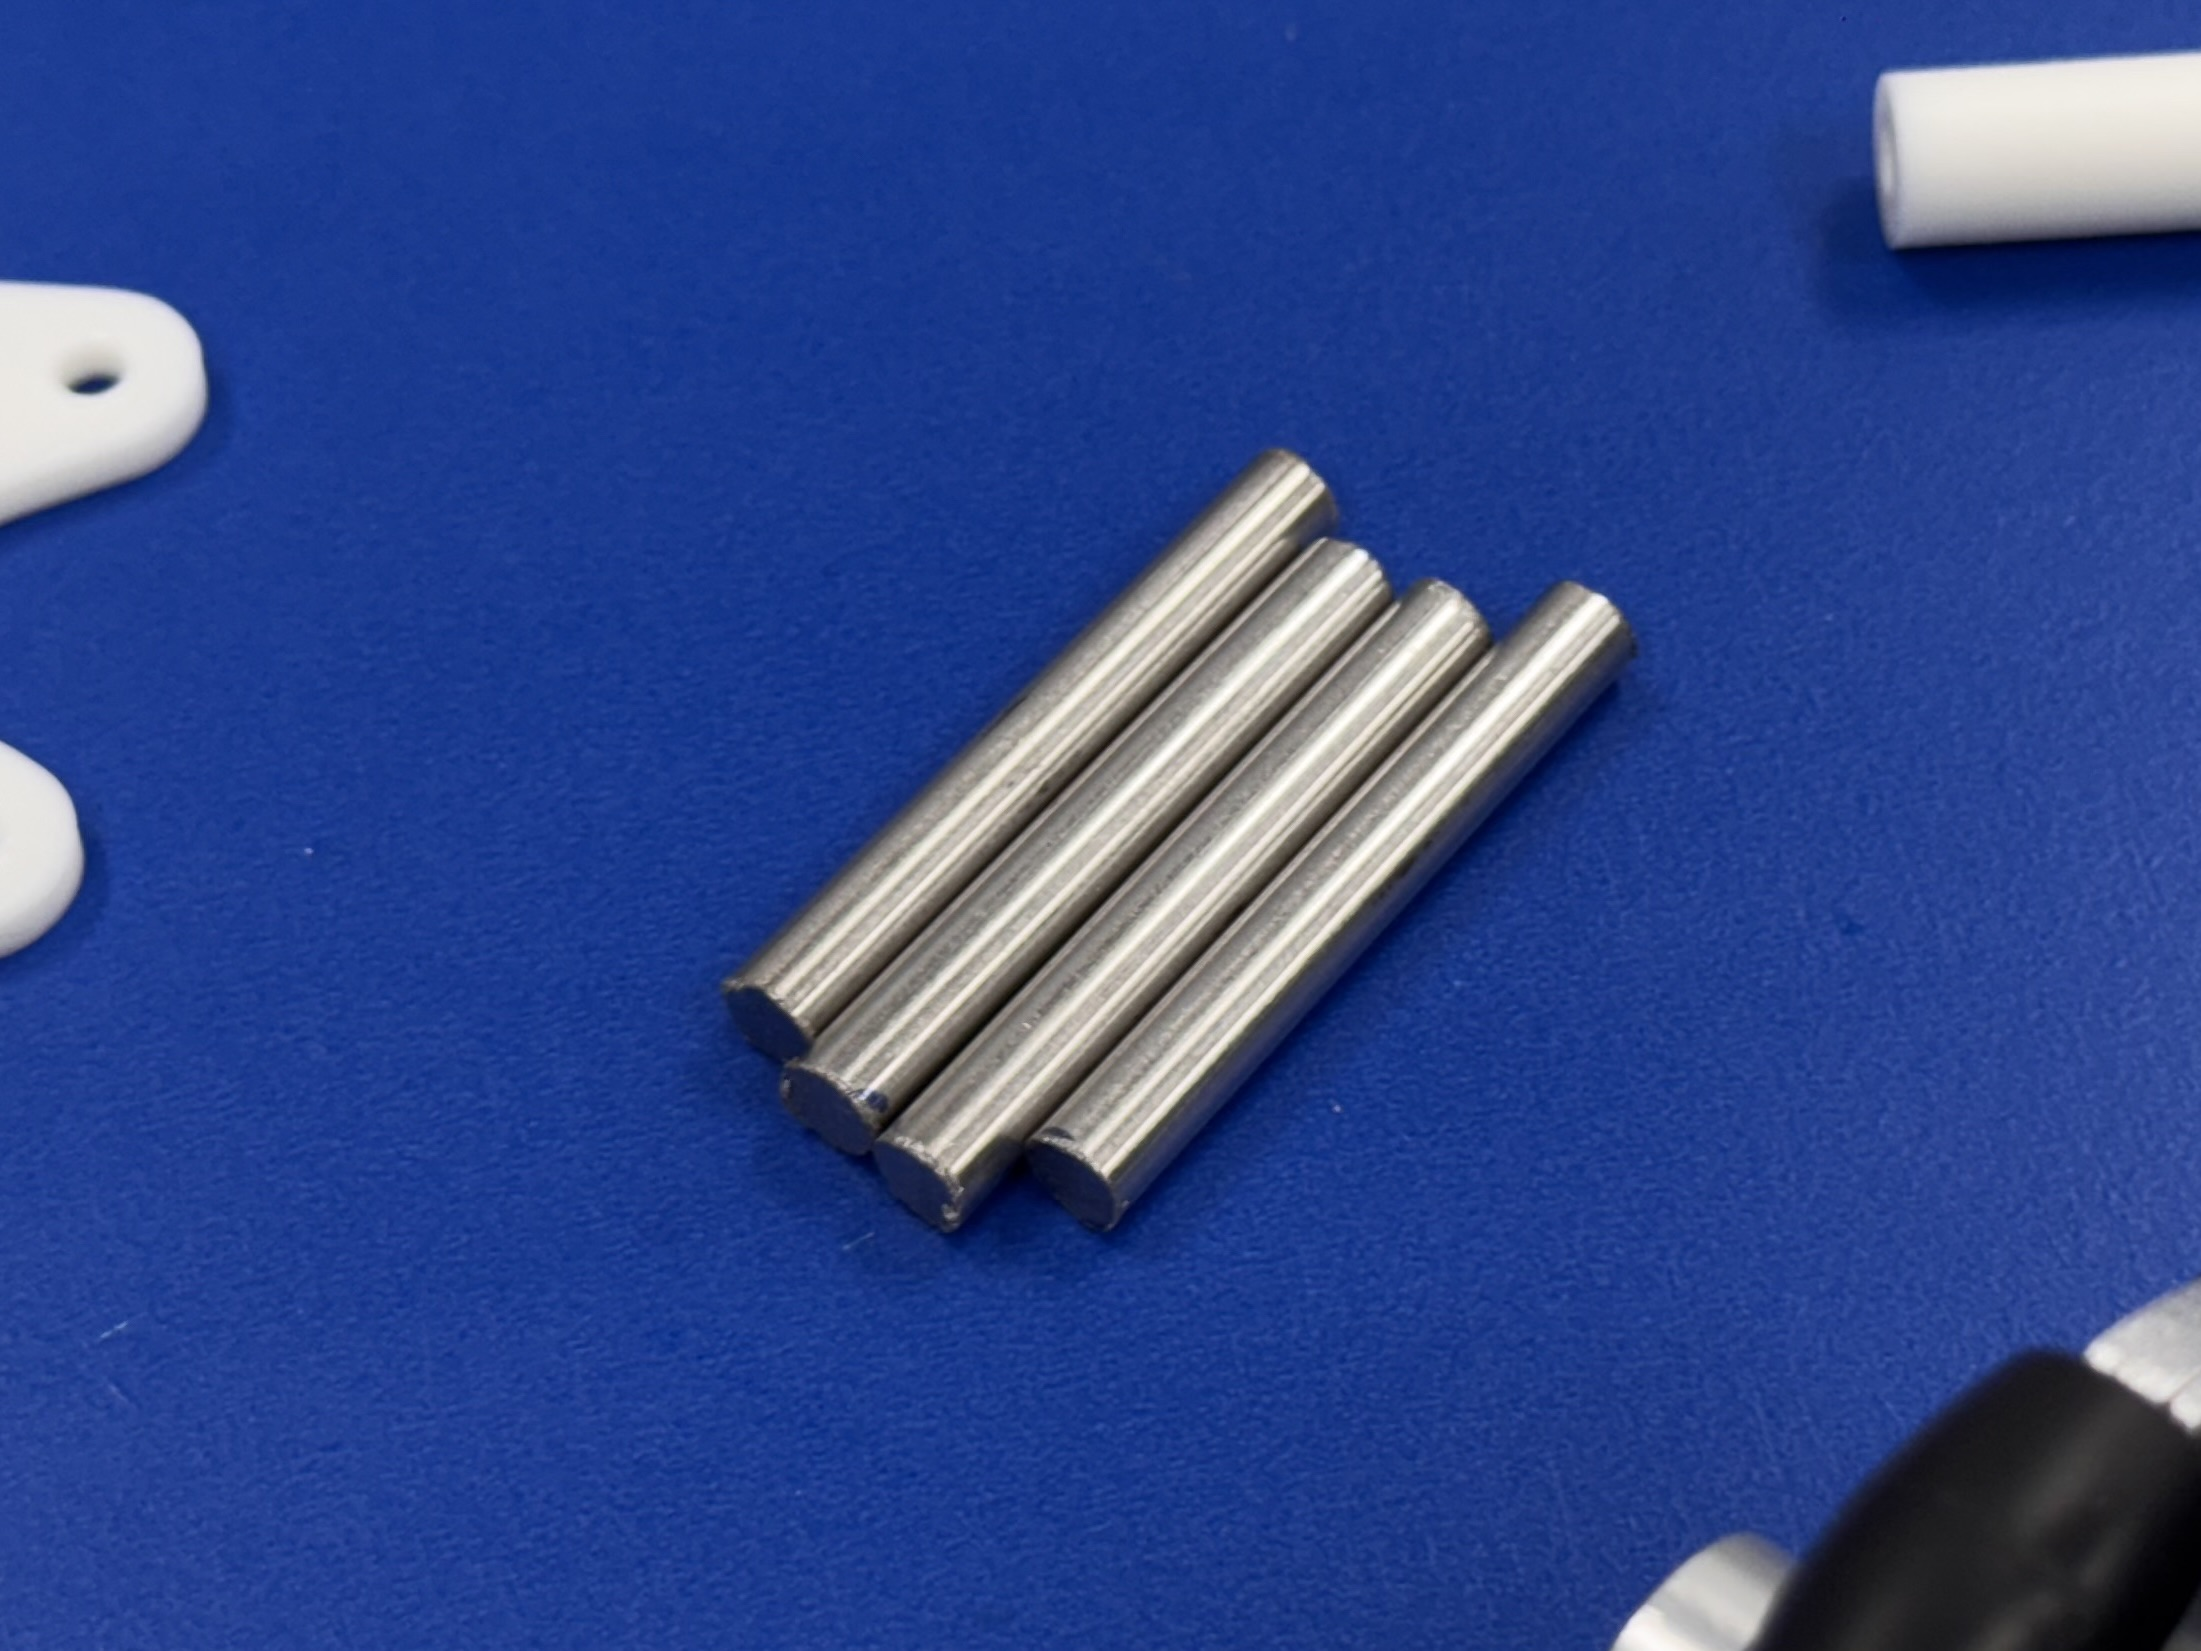
\includegraphics[width=0.5\textwidth]{assets/images/hardware/IMG_8280.jpeg} &
        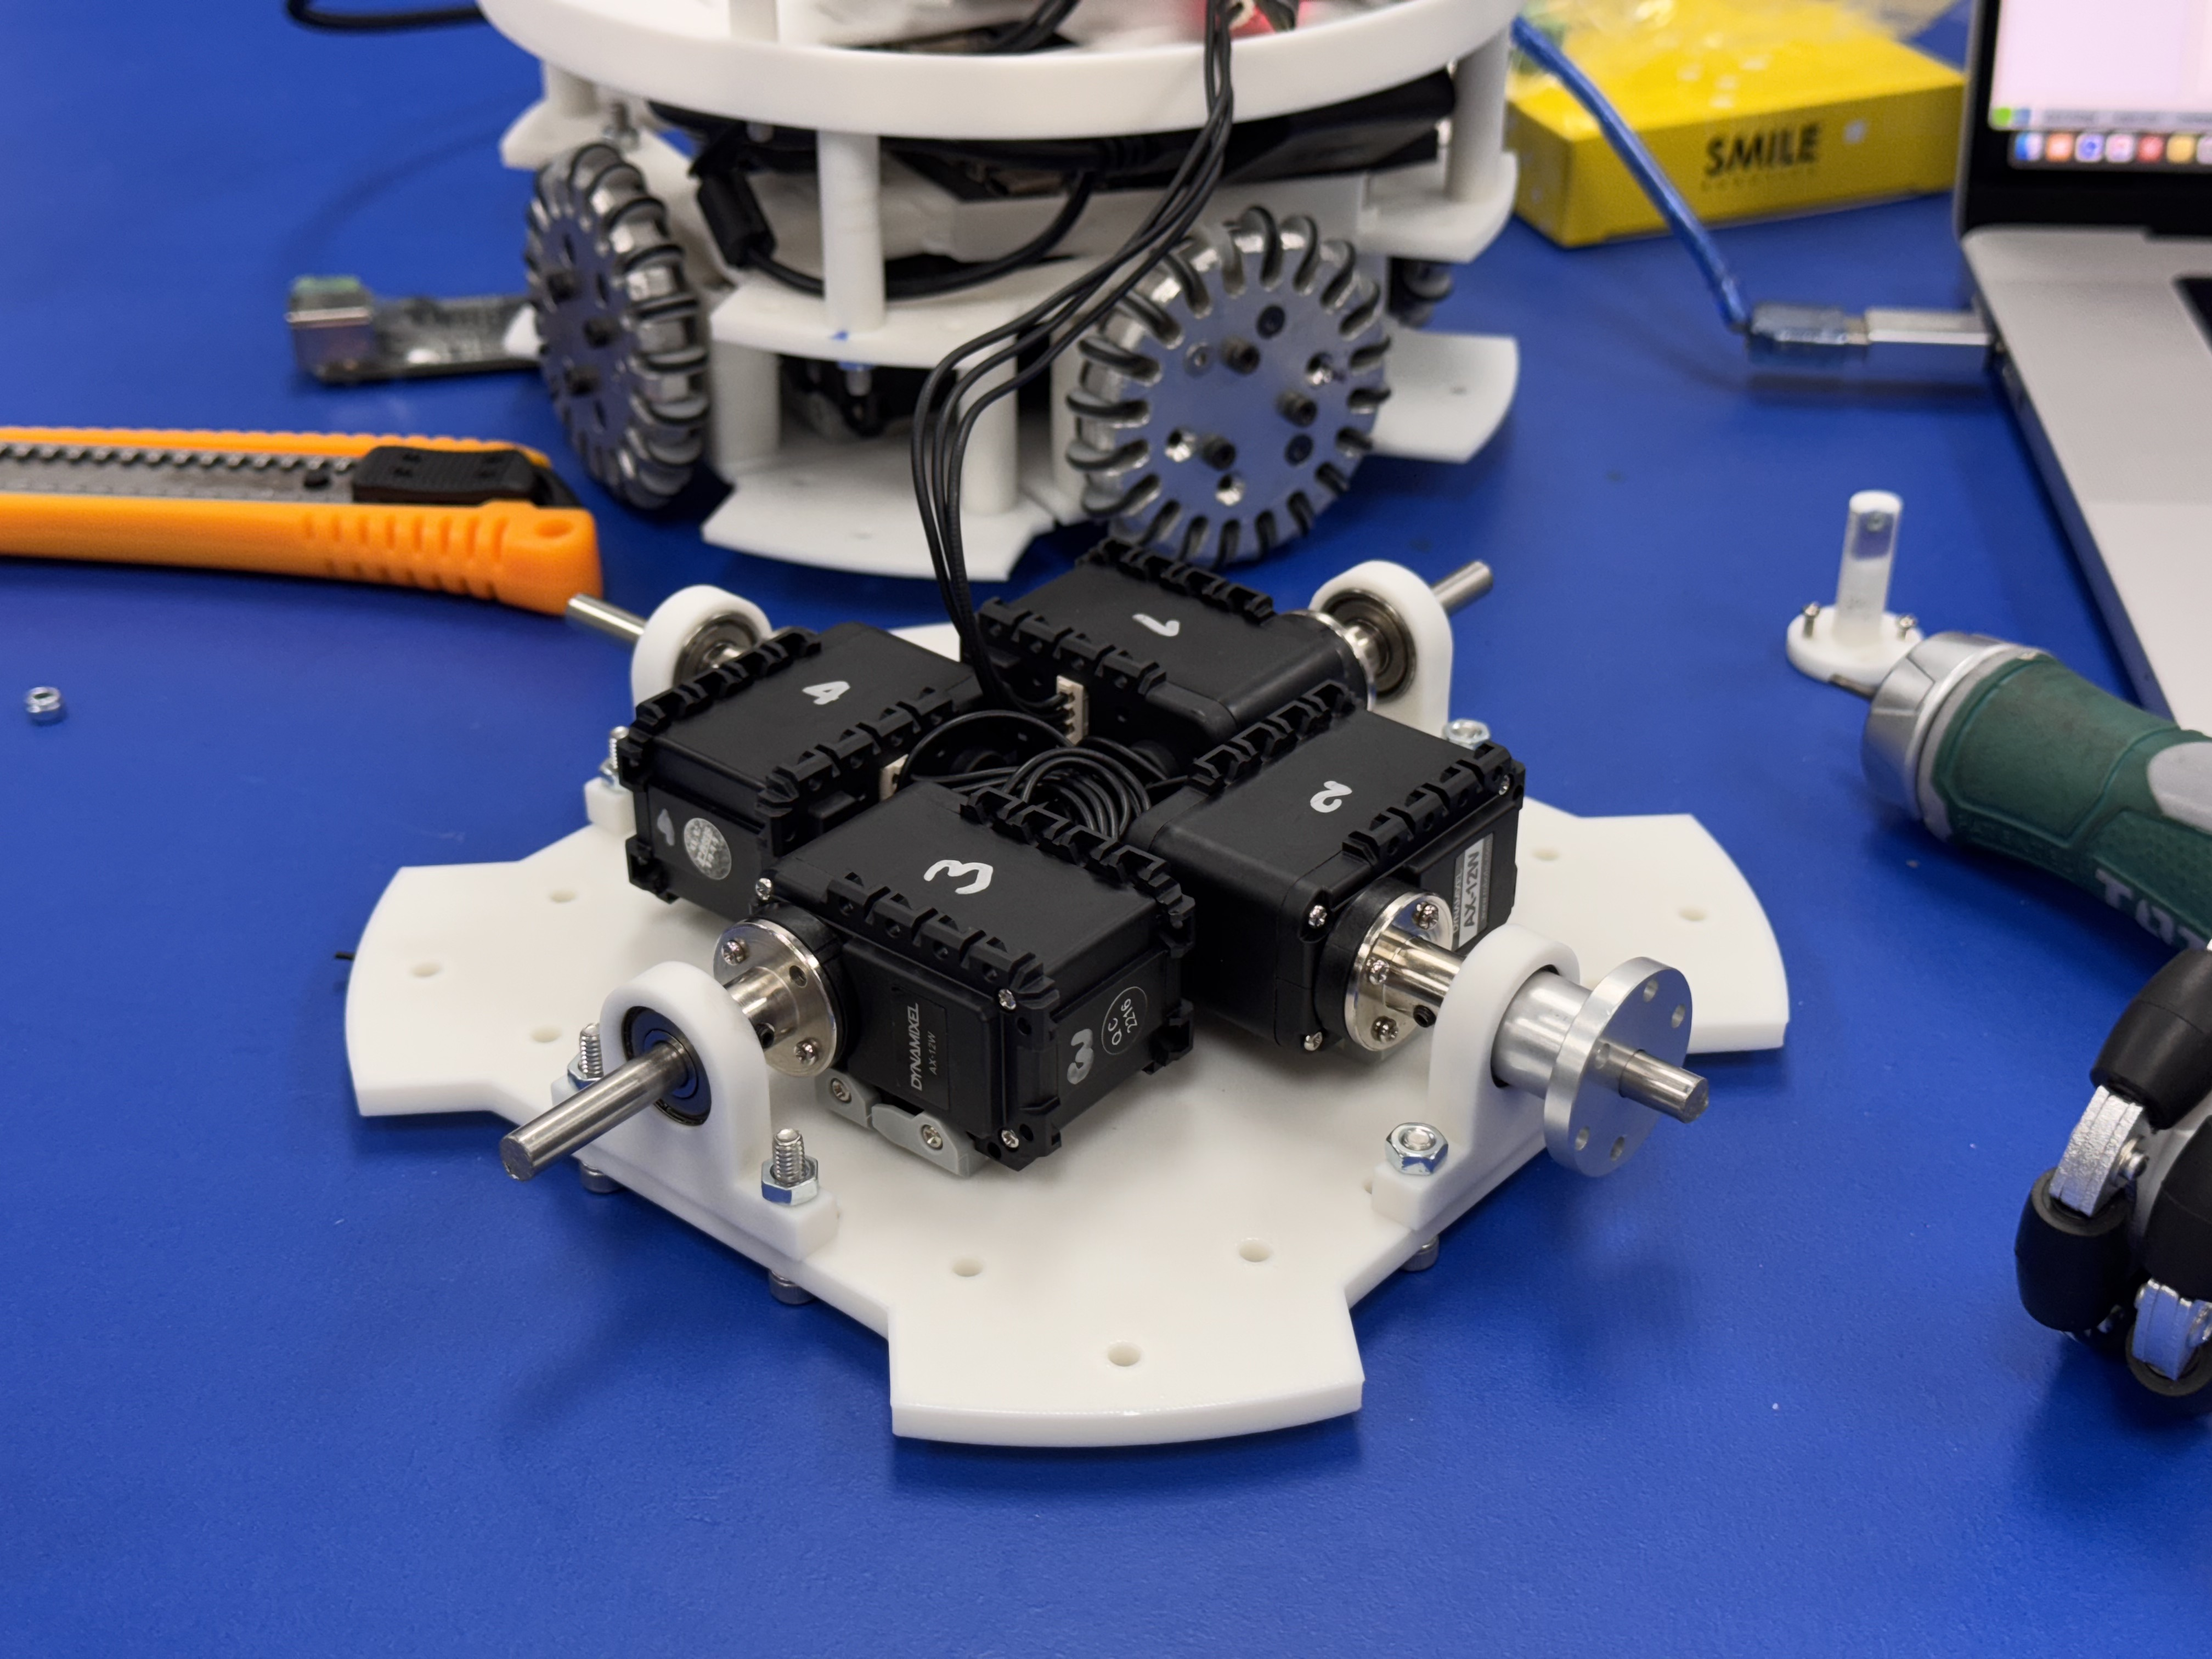
\includegraphics[width=0.5\textwidth]{assets/images/hardware/IMG_8284.jpeg} & \\
        \small Metal Shafts &
        \small Assembly of the motors, motor flange, bearing pillow block, omni-wheel flange&
    \end{tabular}
    \caption{Holonomic movement capabilities of the robot}
    \label{fig:hdinfo-1}
\end{figure}
\begin{figure} [H]
    \centering
    \begin{tabular}{@{}c@{\hspace{0.5cm}}p{8cm}@{\hspace{0.5cm}}c@{}}
        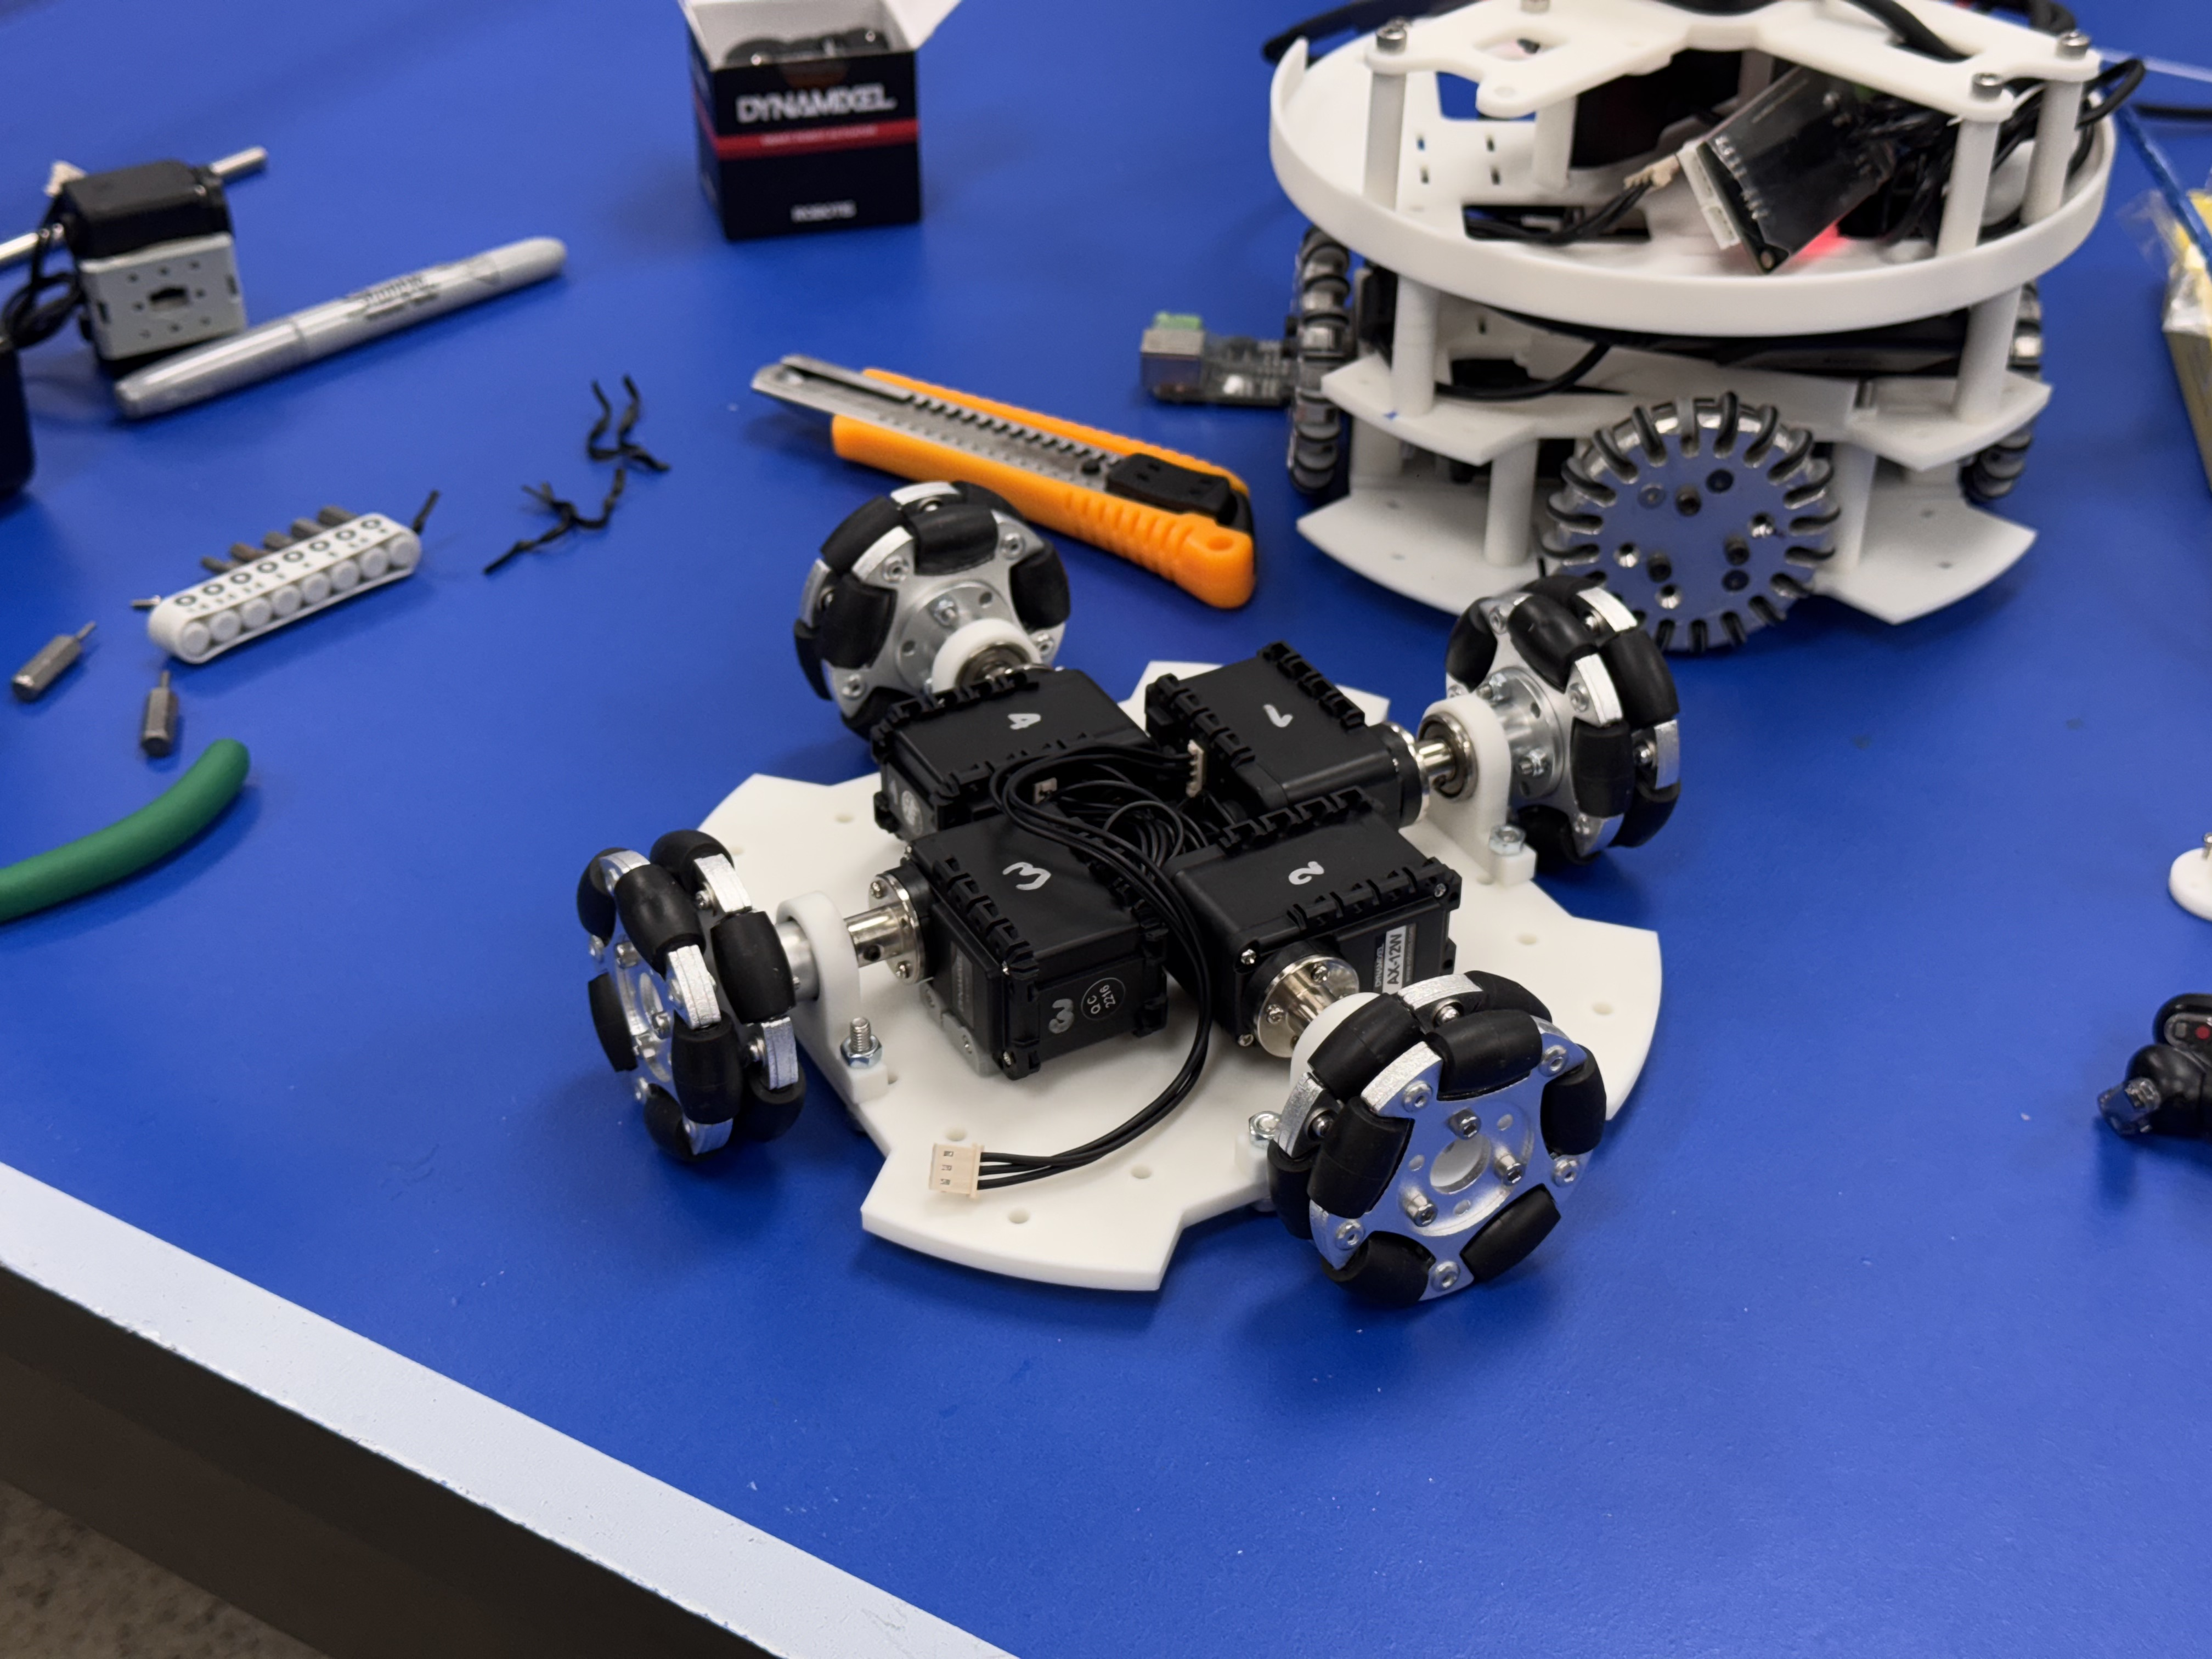
\includegraphics[width=0.5\textwidth]{assets/images/hardware/IMG_8286.jpeg} &
        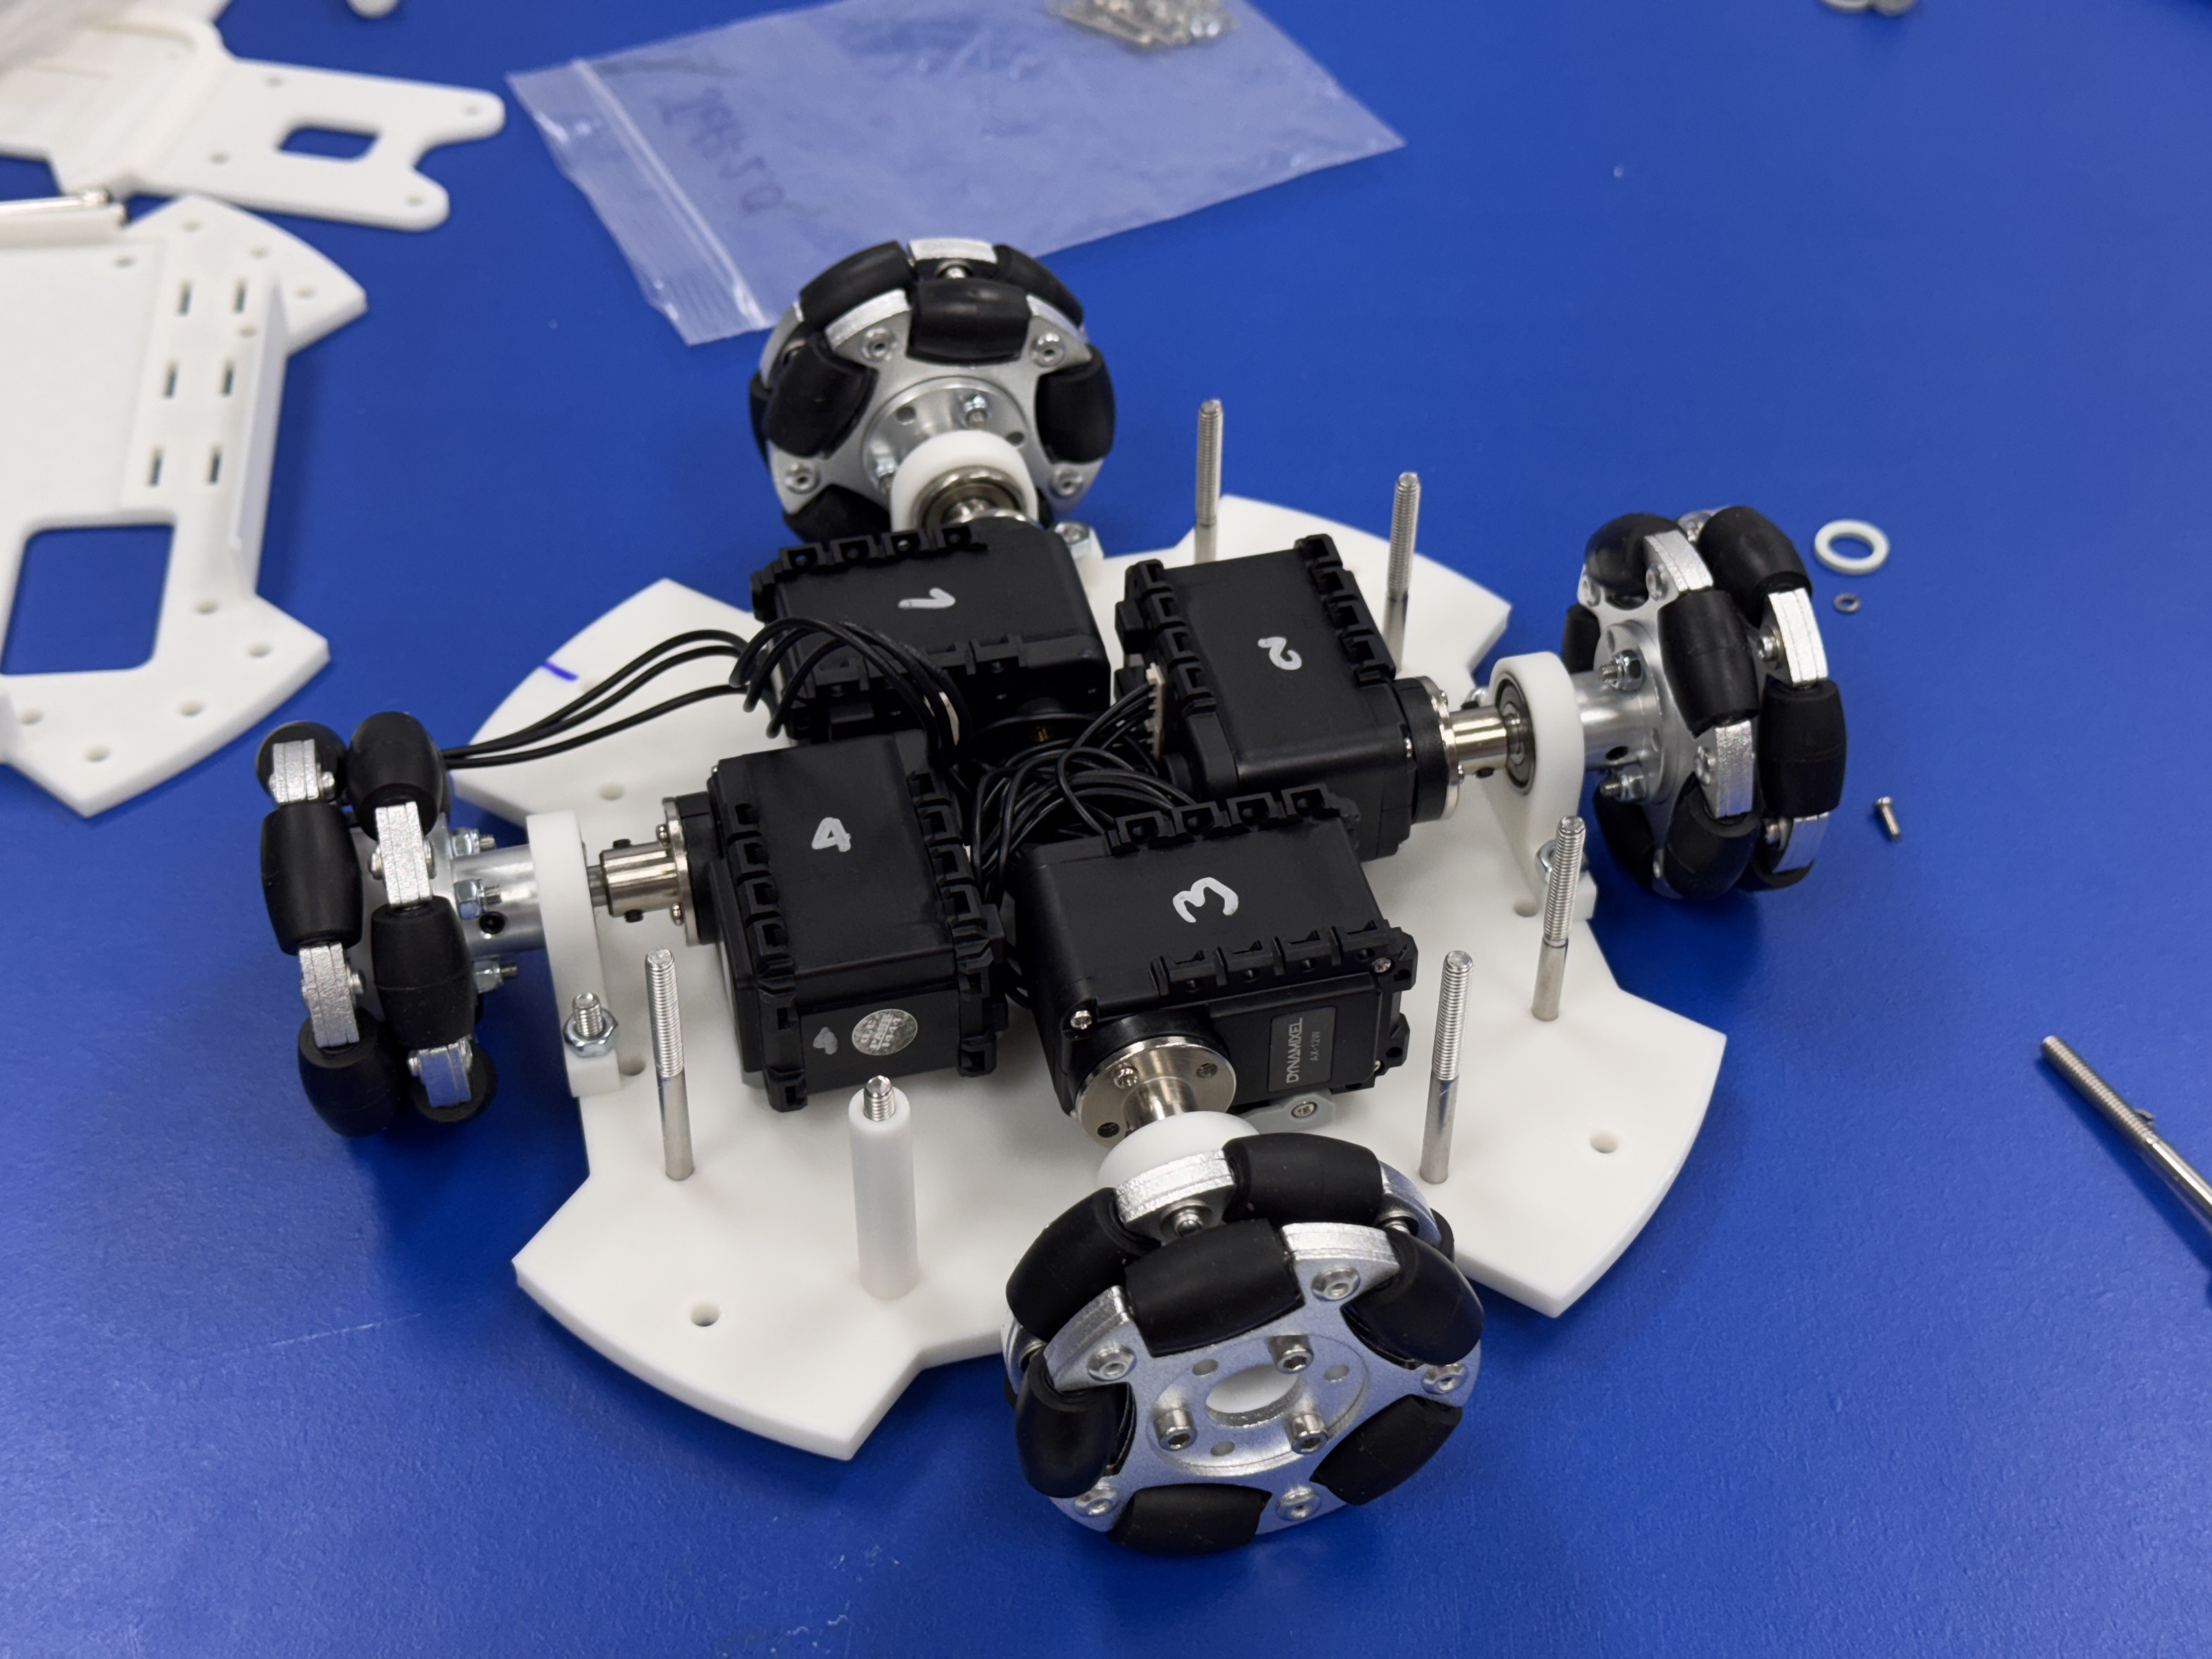
\includegraphics[width=0.5\textwidth]{assets/images/hardware/IMG_8287.jpeg} & \\
        \small Asemmbly of \ref{fig:hdinfo-1}(right) with omni-wheel attached  &
        \small Asemmbly of \ref{fig:hdinfo-1}(right) with omni-wheel attached + standoffs + screws &
    \end{tabular}
    \caption{Holonomic movement capabilities of the robot}
    \label{fig:holo-movement}
\end{figure}
% 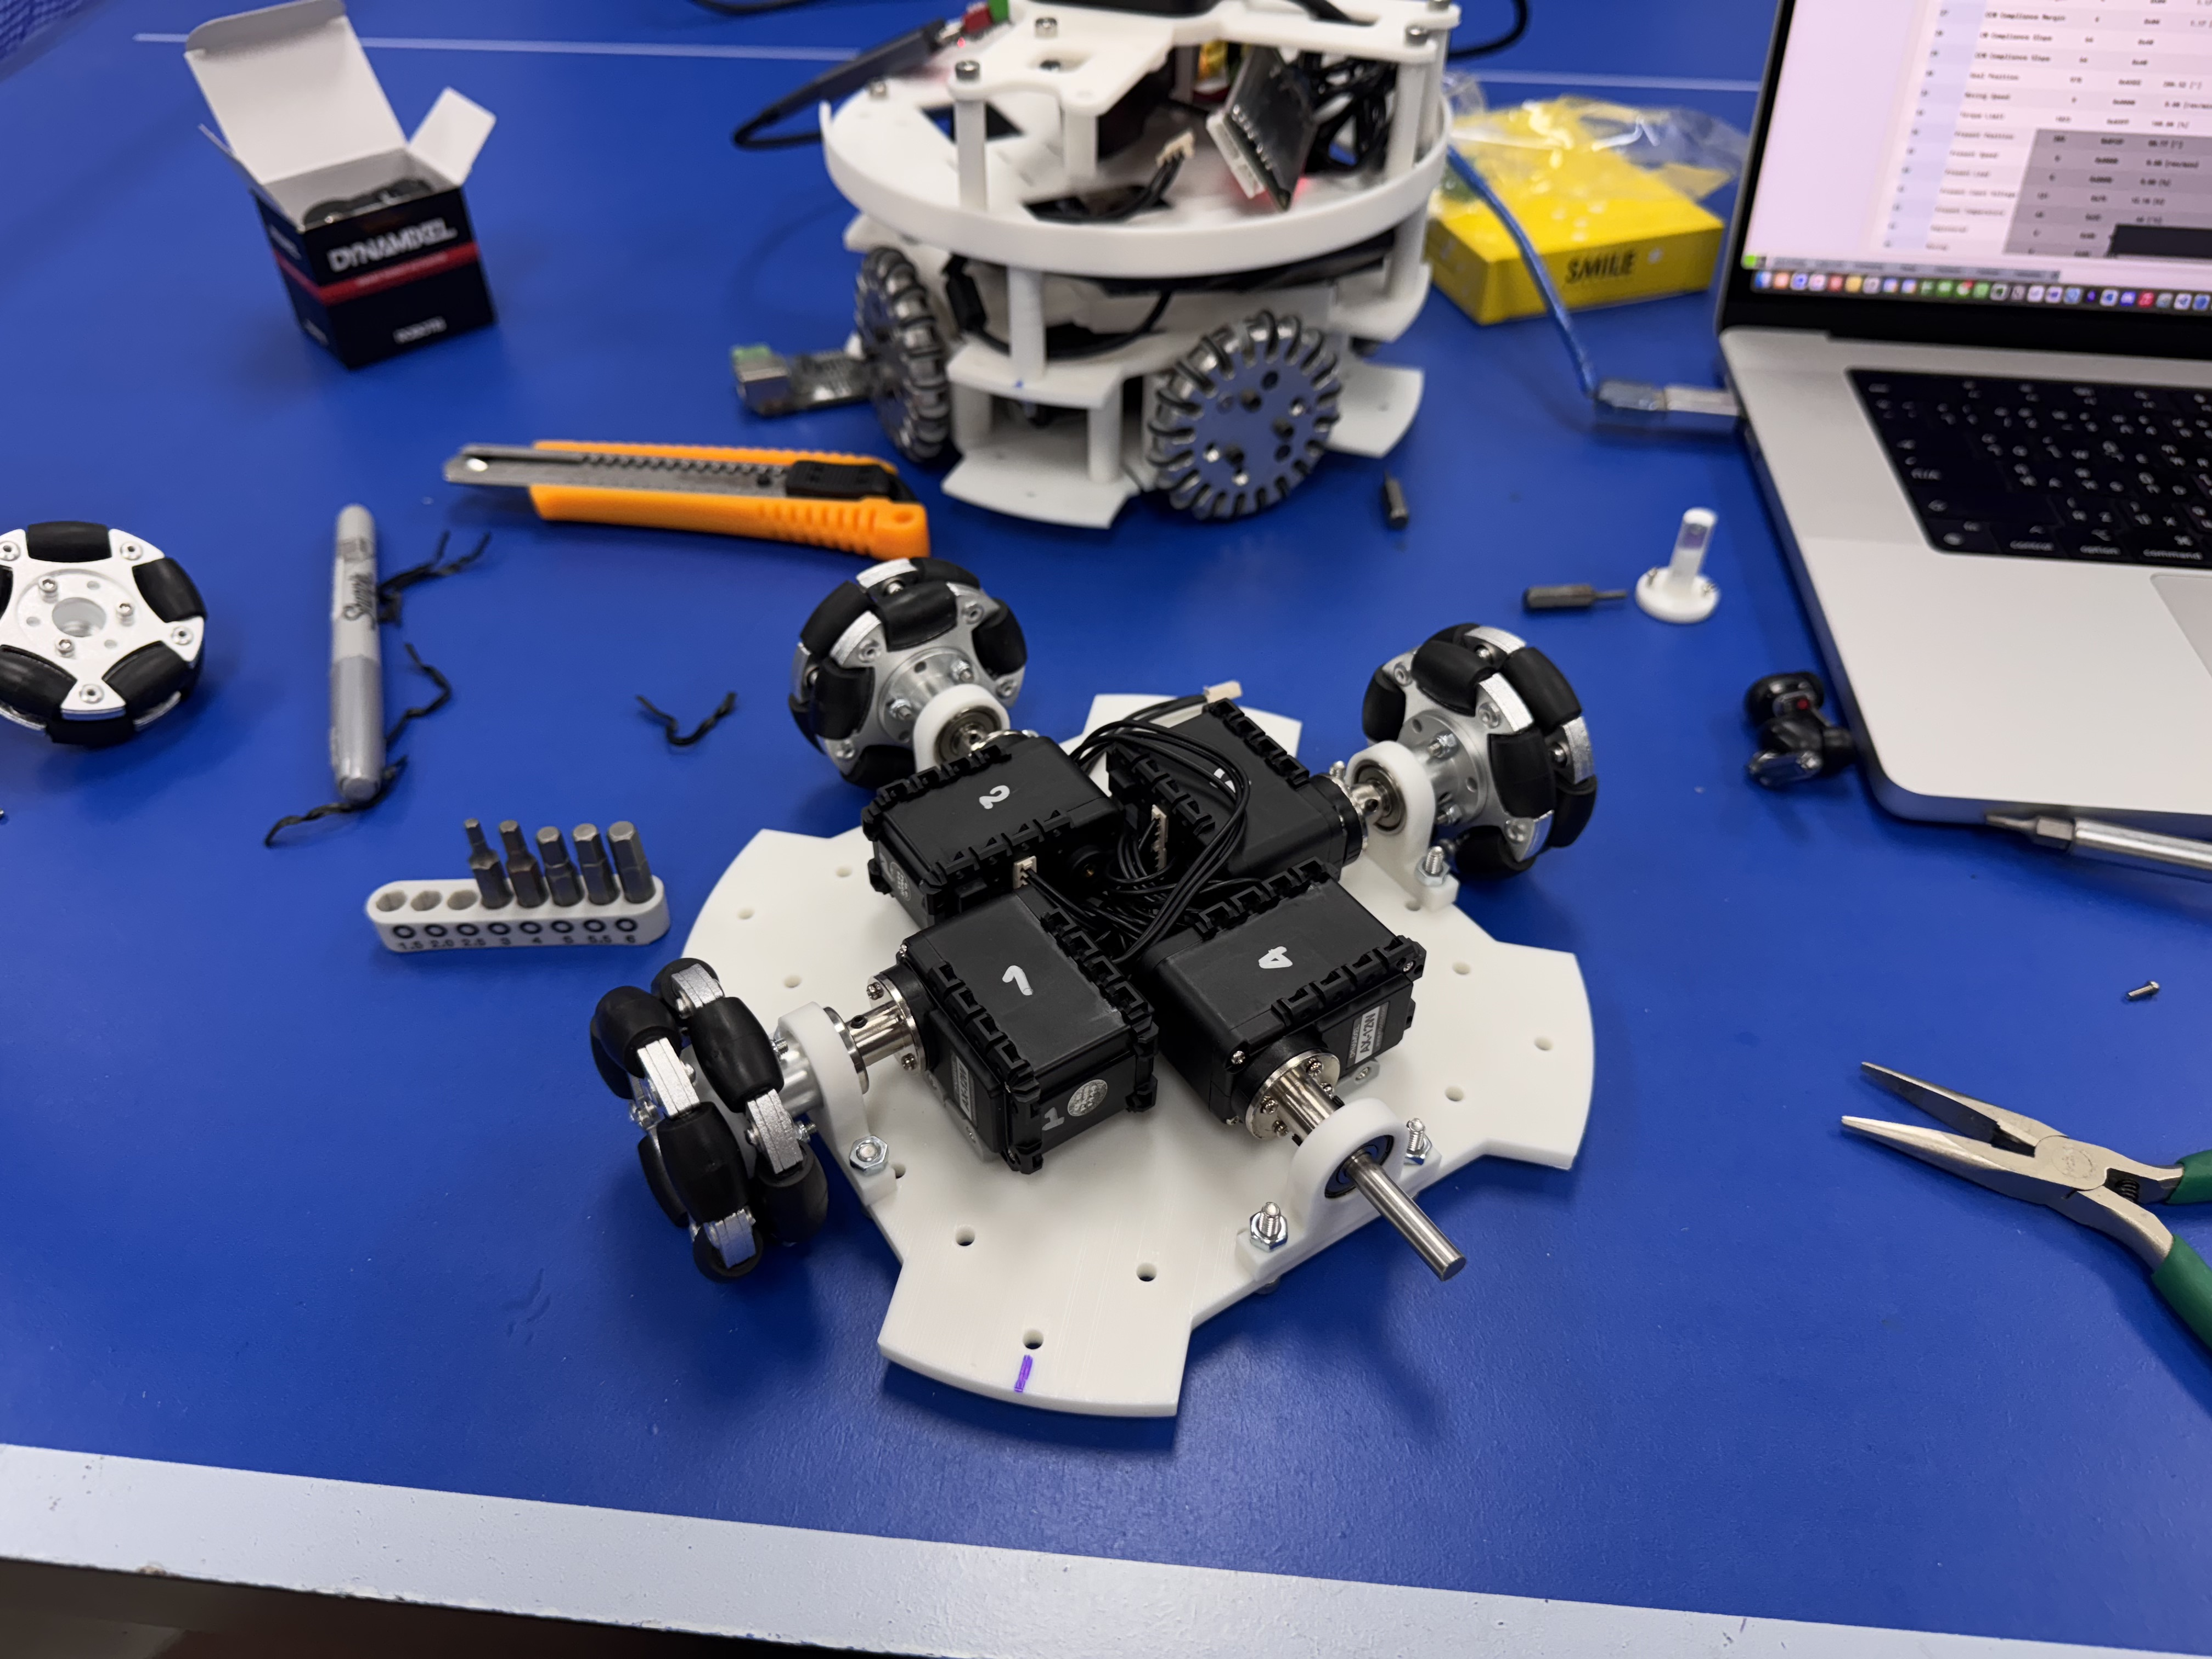
\includegraphics[width=0.3\textwidth]{assets/images/hardware/IMG_8285.jpeg} \\
% \small  \\
The metal shaft in \ref{fig:metal-parts}(left) are cut to equal length to be attached to the flange. This change from PLA plastic helped to reduce the wobble using the 3D printed shaft as they are deform while screwing the lock screw at the wheel flange.

